\documentclass[sigconf,review,anonymous]{acmart}
%\usepackage{draftwatermark}
%\SetWatermarkText{Draft}
\usepackage{balance}
\setcounter{tocdepth}{3}
%\usepackage{cite}
\usepackage{graphicx}
%\usepackage{showframe}
\usepackage{enumitem}
\usepackage[skins]{tcolorbox}

\usepackage{colortbl}
\usepackage{arydshln}
\usepackage{times}
%\usepackage[dvipsnames]{xcolor}
\usepackage{rotating}
\usepackage{makecell}
\usepackage{tabularx}
\usepackage{booktabs}
\usepackage{wrapfig}
\usepackage{tikz}
\usetikzlibrary{angles}
\usepackage{makecell}
\usepackage{tabu}
\usepackage{multirow}
\usepackage{hyperref}
\usepackage{framed} 
\usepackage{newtxtext,newtxmath,amsmath}
\usepackage[framemethod=tikz]{mdframed}
\usetikzlibrary{shadows}
\usepackage{graphics}
\newmdenv[
tikzsetting= {fill=gray!10},
linewidth=1pt,
roundcorner=2pt,
shadow=false
]{myshadowbox}
%\usepackage[framed]{ntheorem}

\newcommand{\bluecheck}{}%
\DeclareRobustCommand{\greencheck}{%
  \tikz\fill[scale=0.25, color=green]
  (0,.35) -- (.25,0) -- (1,.7) -- (.25,.15) -- cycle;%
}
\usepackage{pifont}% http://ctan.org/pkg/pifont
\newcommand{\cmark}{\ding{51}}%
\newcommand{\xmark}{\ding{55}}%

\newenvironment{result}[2]
{\begin{myshadowbox}\textbf{\textit{\underline{Lesson#1:}}} #2}{
\end{myshadowbox}}

\makeatletter
\let\th@plain\relax
\makeatother

\hypersetup{
    linkcolor=blue,
    filecolor=magenta,      
    urlcolor=cyan,
}
\newcommand{\tikzhighlightanchor}[1]{\ensuremath{\vcenter{\hbox{\tikz[remember picture, overlay]{\coordinate (#1 highlight \arabic{highlight});}}}}}

\setlist[itemize]{leftmargin=0.4cm}
\setlist[enumerate]{leftmargin=0.4cm}

\newcommand{\bi}{\begin{itemize}}
\newcommand{\ei}{\end{itemize}}
\newcommand{\be}{\begin{enumerate}}
\newcommand{\ee}{\end{enumerate}}
\newcommand{\fig}[1]{Figure~\ref{fig:#1}}
\newcommand{\eq}[1]{Equation~\ref{eq:#1}}
\newcommand{\tion}[1]{\S\ref{sect:#1}}

\newenvironment{RQ}{\vspace{1mm}\begin{tcolorbox}[enhanced,width=3.4in,size=fbox,colback=red!5!white,drop shadow southwest,sharp corners]}{\end{tcolorbox}}

\usepackage{url}
%\newcommand{\keywords}[1]{\par\addvspace\baselineskip \noindent\keywordname\enspace\ignorespaces#1}
%%% graph
\newcommand{\crule}[3][darkgray]{\textcolor{#1}{\rule{#2}{#3}}}

\tikzstyle{thmbox} = [rectangle, rounded corners, draw=black, fill=gray!10]
\newcommand\thmbox[1]{%
	\noindent\begin{tikzpicture}%
	\node [thmbox] (box){%
		\begin{minipage}{.94\textwidth}%
		\vspace{-0.1cm}#1\vspace{-0.1cm}%
		\end{minipage}%
	};%
	\end{tikzpicture}}

\newcommand{\quartex}[4]{
\begin{picture}(25,6)%1
    {
        \color{black}
        \put(#3,3)
        {\circle*{4}}
        \put(#1,3)
        {\line(1,0){#2}}
    }
\end{picture}
}

\acmConference[ESEC/FSE 2020]{The 28th ACM Joint European Software Engineering Conference and Symposium on the Foundations of Software Engineering}{8 - 13 November, 2020}{Sacramento, California, United States}

\title[Changing  Nature of CS Software]{The Changing Nature of Computational Science Software}
\author{Huy Tu, Rishabh Agrawal, Tim Menzies}
\affiliation{ Computer Science, NC State, USA} \email{hqtu@ncsu.edu,  ragrawa3@ncsu.edu, timm@ieee.org}
%
%
\date{December 2019}


\begin{abstract}

The use of computational software for scientific discovery
has increased recently. Yet, how Software Engineering can be adapted for Computational Science (CS) is still puzzling to both communities. 

Prior studies that stress the need for understanding scientific software development are qualitative in nature and possibly applicable at a particular point in the history. A recent trend within CS is  
%in that community is that, increasingly,
the source codes are being stored in pubic domain repositories such as Github.
Hence, it is now possible to explore
the characteristics of scientific software development using
that public domain data.
This paper accordingly seek quantitative evidence (from 59 CS projects housed in Github) for
  13 previously published
  conjectures about   CS projects in the literature. In all, we explore
  three groups of beliefs about
    (1)   the
nature of scientific challenges; (2) the implications of  limitations of computer hardware; and (3)  the cultural environment of scientific software development. 
We find that three beliefs cannot be assessed
with respect to the Github data. Of the others, only four can be endorsed. 

More than half of the deep-rooted beliefs were  doubted,  which lead us to conclude that the
nature of CS software development is
changing. This has design implications that the tools we develop to support software-based-science and the debate around that need to be updated as new data is available.



\end{abstract}
 
\keywords{Computational Science, Software Engineering}

\begin{document}


\maketitle
\section{Introduction}
%TODO: It is from our observation that (1) requirements and (2) testing are only low-hanging fruits within the CS community. It is essential for us to do more in-depth analysis of the development code base and social interaction (e.g. mailing lists, issues/commits comments, commit's message, etc) to understand the community.  

Computational Science (hereafter, CS)
uses software   to explore
 astronomy, astrophysics, chemistry, economics, genomics, molecular biology, oceanography, physics, political science,  and many   engineering fields 
CS is becoming more dependent on software. For instance, a Nobel Prize in 2013 went to chemists using computer models to explore chemical reactions during photosynthesis. In the press release of the award, the Nobel Prize committee wrote:
\begin{quote}
{\em Today the computer is just as important a tool for chemists as the test tube \cite{nobel_2013}.}
\end{quote}

If we can better understand the nature of the
software development practices in CS
then we would be better at improving those methods and alleviating some of the effort involved in sustainability, verifiability, reproducability, comprehension, and usability of those software.
Improving (say) the 
 maintainability of CS code
 can elevate productivity of scientific research in the following ways: 
(1) the adaptation of scientific projects simulations to new and efficient hardware  (multi-core and heterogeneous systems); (2) the ability for larger teams to co-ordinate (through integration with interdisciplinary teams); and (3) how well we can model complex phenomena. 
%  \bi
%  \item
%  The adaptation of scientific projects simulations to new and efficient hardware  (multi-core and heterogeneous systems);
%  \item The ability for larger teams to co-ordinate (through integration with interdisciplinary teams);
%  \item How well we can model complex phenomena.
%  \ei
 

 
 Note that we are not the first to stress the need for better SE for CS. The quality of scientific software through the ``Climategate'' scandal \cite{merali10_error} uncovered a lack reproducibility of CS results. Improving the verifiability of CS code would hence increase the   credibility of results from  CS research. 

\definecolor{carnationpink}{rgb}{1.0, 0.65, 0.79}
\newcommand{\DOUBT}{\colorbox{carnationpink}{{\bf Doubt}}}

\definecolor{celadon}{rgb}{0.67, 0.88, 0.69}

\newcommand{\ENDORSE}{\colorbox{celadon}{{\bf Endorse}}}
\begin{table*}[t]
\centering
\vspace{-0.15cm}
\resizebox{0.83\linewidth}{!}{

%\begingroup\setlength{\fboxsep}{2pt}
%\colorbox{lightgray}
%
\begin{tabular}{c|l|l|c}
Category  & Characteristics & Citations & Conclusion \\ \hline

\multirow{3}{*}{\begin{tabular}[l]{@{}c@{}c@{}} 1. nature of \\ scientific  \\ challenge\end{tabular}}  &  \multirow{3}{*}{\begin{tabular}[c]{@{}l@{}l@{}} a) Requirements are Not Known up Front 
 \\ b) Verification and Validation are Difficult and Strictly Scientific 
 \\ c) Overly Formal Software Processes Restrict Research 
\end{tabular}}
& \cite{segal08_ss, carver07_environment, segal05_ss, basili08_hpc, easterbrook_cs} & \ENDORSE \\
& & \cite{carver07_environment, kanewala13_testing, carver06_hpc, Prabhu11_cssurvey, basili08_hpc} & \ENDORSE  \\
& & \cite{easterbrook_cs, segal07_problem, carver07_environment, segal08_ss} & No-Evidence \\ \hline

\multirow{4}{*}{\begin{tabular}[l]{@{}c@{}c@{}c@{}} 2. limitations \\ of computer \\ hardware \end{tabular}}  &  \multirow{4}{*}{\begin{tabular}[c]{@{}l@{}l@{}l@{}} a) Development is Driven and Limited by Hardware & 
 \\  b) Use of ``Old'' Programming Languages and Technologies 
 \\ c) Intermingling of Domain Logic and Implementation Details 
 \\ d) Conflicting Software Quality Requirements 
\end{tabular}} 
 & \cite{easterbrook_cs, faulk09_secs} & No Evidence \\
 & & \cite{basili08_hpc, carver07_environment, Prabhu11_cssurvey, kendall05_C, ragan14_pythoncs} & \DOUBT \\
 & & \cite{faulk09_secs} & \ENDORSE \\
 & & \cite{carver07_environment, basili08_hpc, carver06_hpc} & No Evidence \\ \hline

\multirow{6}{*}{\begin{tabular}[l]{@{}c@{}c@{}c@{}c@{}c@{}} 3. limitations \\ of cultural \\ differences \end{tabular}}  &  \multirow{6}{*}{\begin{tabular}[c]{@{}l@{}l@{}l@{}l@{}l@{}} a) Different Terminology 
 \\ b) Creating a Shared Understanding of a ``Code'' is Difficult 
 \\ c) Little Code Reuse 
 \\ d) Scientific Software in Itself has No Value But Still It is Long-Lived 
 \\ e) Few Scientists are Trained in Software Engineering
 \\ f) Disregard of Most Modern Software Engineering Methods 
\end{tabular}} 
 &  \cite{faulk09_secs, easterbrook_cs, boyle09_lessons} & \ENDORSE \\
 & & \cite{segal07_problem, carver06_hpc, Shull05_parallel, sanders08_risk} & \DOUBT \\
 & & \cite{Prabhu11_cssurvey, segal07_problem, basili08_hpc, carver06_hpc} & \DOUBT \\
 & & \cite{faulk09_secs, segal07_enduser, easterbrook_cs, boyle09_lessons} & \DOUBT \\
 & & \cite{segal07_enduser, basili08_hpc, carver13_perception, easterbrook_cs, sanders08_risk} & \DOUBT \\ 
 & & \cite{carver13_perception, hannay09_secs, Prabhu11_cssurvey, carver06_hpc, boyle09_lessons} & \DOUBT \\
\end{tabular}}
\caption{Thirteen beliefs from
prior studies about Computational Science. From Johanson et al. \cite{johan18_secs}. These beliefs
divide into the three categories shown in the left-hand column.
In the far right column,
anything marked as ``no evidence''
refers to beliefs we could
not check using our Github data.}
\label{tab:characteristics}
\vspace{-20pt}
\end{table*}



Table \ref{tab:characteristics}
lists some of the prior results
where empirical software
engineering researchers have explored computational science
(this table comes from the work of
Carver, Heaton, Basili, and Johanson \cite{carver13_perception, carver07_environment, basili08_hpc, heaton15_lit, johan18_secs}, and others).
Johanson et al. \cite{johan18_secs}   argues that SE practices will only be integrated into CS if the honor the 13 beliefs listed in
Table \ref{tab:characteristics}. Yet, issues with much of the analysis of Table \ref{tab:characteristics} are such analysis is often applied to (1) just a handful of projects (or even, just one); (2) is often qualitative in nature; and (3) only some are relevant at a particular time. Hence, that prior work does not lend itself to being double-checked by subsequent studies that survey numerous projects. 


Given the relevance of CS field, prominence of the beliefs
from Table \ref{tab:characteristics}, and the limitations of prior studies, it is important to assert the prevalence of these beliefs with empirical evidence. A recent trend is that CS researchers store their code on opens source repositories (such as Github). This study mines the code and comments of dozens of those repositories, to assess the current relevance of the Table \ref{tab:characteristics}'s beliefs. This approach built on \textit{indicators} -  measure or metric that evaluates goal with respect to some objectives. To illustrate, suppose you are assessing how delicious a dish is without tasting it. The fragrance's strength, the color, the arrangement, and the distribution of meat and veggies from the dish can serve as \textit{indicators} for your estimation of the dish's deliciousness. In the same vein, for each belief in this study:
\be
\item We constructed observable indicators and conditions of how indicators should be if the belief was true.   
\item We endorse/doubt that belief if those conditions are met/unmet within the Github CS repositories.
\ee

Each of these beliefs is essential to the future of interdisciplinary of both CS and SE fields. Our study goal is not to thoroughly cover and investigate all the corner cases existing in each belief which would not serve them justice. However, our goal is to report on if these beliefs are still hold in respect to the empirical indicators from the accessed data. Therefore, an important part of this analysis is that all of our reasonings are repeatable/ refutable/ improvable e.g. scales to multiple projects and can be tested by anyone with access to Github.
Based on the analysis of 59 CS projects, we found that:
\bi
\item Three out of 13 beliefs cannot be assessed using Github data: 1c, 2a, \& 2d. 
\item Of the other ones, we can endorse four of them:  1a-b, 2c, \& 3b.
\item But we must doubt the rest six beliefs: 2b, 3a, \& 3c-f. 
\ei

Our results are not refuting deep-rooted CS experts' beliefs but acknowledging that an important aspect of research and the evolving nature of CS require reassessing these beliefs whenever new data is available. We provide some implications for future debate and supporting tools for software-based-science 

% This is not to say that six of the beliefs of  Table \ref{tab:characteristics} are wrong.
% Rather we would say that the nature of CS is ever evolving and that old
% beliefs needs to be rechecked  
% With the changing state of scientific software development, we should also evolve the tools we use to support software-based-science and the debate around that. 


% is that true? Can we audit those
% beliefs

% mentioned in the 
% It is inevitable that the two fields must not continue existing in isolation. However, the gap bridging progress of modern SE practices in computational science has remained status quo through 13 recurring underlying causes results from the nature of scientific challenges, from limitations of computers, and from the cultural environment of scientific software development that developed and restated through this past decade by  


% Orior researchers 
% There have been definite efforts in employing these modern SE practices - which was proven to improve the traditional software - for the CS field. This hopefully would be of great assistant to the computational scientists in the fields such as molecular dynamics, quantum chemistry, and computational materials. However, there have not been large scale empirical study and results indicating the validity of these improvement observations while recommending actionable changes for these observations to hold in the scientific context.       

% It is important first to identify and understand how scientific software development differentiates from Software Engineering (hereafter, SE) development. Faulk et al. and Hannay et al. \cite{hannay09_secs, faulk09_secs} note that a ``wide chasm'' of how these two fields are speaking a common language, yet ``separated'' by upholding to a different cultures and values:
% \bi
% \item
% Software development practice has aimed for generality of ``all things applied'' perplexing computational scientists focusing on ``domain specific''. 

% Consequently, the rift between these two fields in communication and collaboration was created and has been growing with both productivity and credibility crisis.



% It is inevitable that the two fields must not continue existing in isolation. However, the gap bridging progress of modern SE practices in computational science has remained status quo through 13 recurring underlying causes results from the nature of scientific challenges, from limitations of computers, and from the cultural environment of scientific software development that developed and restated through this past decade by Carver, Heaton, Basili, and Johanson \cite{carver13_perception, carver07_environment, basili08_hpc, heaton15_lit, johan18_secs}. Johanson et al. \cite{johan18_secs} specifically claims that SE practices will only be integrated if they honored the mentioned 13 characteristics and constraints of scientific software development mentioned in the Table \ref{tab:characteristics}.
% Traditional SE environments such as businesses or IT companies have used SE practices, it is puzzling of how the scientific software developers not using them or not using them effectively. Throughout literatures, there have not been a quantitative study of these 13 characteristics and constraints in order to give a more empirical view of the scientific software development practices in comparison with the traditional SE practices. 

 
 

\section{Preliminaries  } 

\subsection{Why Study CS (Computational Science)?}

CS scientists study and develop software that have important and widespread impacts to our society.  
For example, weather forecasts generated from CS
software can  predict the path of hurricanes. This, in turn,
allows (e.g.) effected home owners to better protect themselves from
damaging winds. In material science, CS explores the properties
of new materials by synthesizing them, which is very expensive so standard practice is to use software to determine
those properties (e.g. via a finite element analysis). This, in turn, enables (e.g.) the faster transition of new materials to industry.

From these examples, there are multiple good reasons for increasing reliance of computational methods software for science such as it is real-time, more precise, faster, cheaper, and safer to 
explore software models than manually explore the physical effects they represent. For instance, CS software can explore the effects of several 
hurricanes 
scenarios and nuclear reactions without risk to  human  life
or property \cite{heaton15_lit}. 

The growing dependency of science on computational methods software to make decisions for scientists is inevitable. By enhancing the software's quality, scientists can guarantee the CS work more credible and more productive. Therefore, 
better SE improves computational
science software, which would lead to better (e.g.) weather  prediction and the faster creation of new industries based on new materials.

\begin{table*}
\caption{  CS projects
 that satisfy
the sanity checks of
Table~\ref{tbl:sanity}.
This list has been auditted by
a domain expert from  CS
(Dr Robert Sinkovits, San Diego
SuperComputer Center  (https://www.sdsc.edu/~sinkovit/)) who commented that   many of these projects account for the majority of the supercomputer usage in computational
science. While some of these  focus on  computational chemistry,  they   also   include  numerous widely-used support tools (e.g
elasticsearch) or simulation tools that are cross-disciplinary (e.g. the classical simulation tools
used  by molecular biologists).  Also, there are also tools here used in material science (e.g. LAMMPS).}
\label{tbl:samples}
{
 \small
\hspace{0.5cm}\begin{tabular}{r|lcccccrrc}
\renewcommand{\baselinestretch}{0.7}
&   &   &   &   &  &  &  & Analyzed \\
% 
 & Language & \# Developers & Duration(Years) & \# Commits & \# Stars & \# Issues & \# Releases  & in Fig.\ref{fig:belief1}\&\ref{fig:SE_activities}\\  
 %& in Figure~2
\hline
\rowcolor{blue!10}  cctools & C	 & 43	& 5.5 & 8881	& 72 & 666 & 159  &  \checkmark \\
keplerproject & C & 22	& 5.25 & 329 & 26 & 66	& 18 &   \\
BLIS & C & 20 & 4.8 & 1242 & 413 & 142 & 25 &   \\\hline 
\rowcolor{blue!10}PCMSolver & C++ & 8 & 4 & 1844 & 13 & 88 & 16 & \checkmark \\ 
\rowcolor{blue!10}AMBER & C++ & 12 & 4 & 8382 & 32 & 249 & 3 & \checkmark\\
\rowcolor{blue!10}HooMD-blue & C++ & 36 & 2.5 & 9450 & 54 & 330 & 25 & \checkmark \\
\rowcolor{blue!10} dealii & C++ & 120 & 18 & 41514 & 382 & 1604 & 26 & \checkmark  \\
\rowcolor{blue!10}  Psi4 & C++ & 79 & 5.5 & 12178 & 247 & 504 &	7 & \checkmark  \\
\rowcolor{blue!10}LAMMPS & C++ & 74 & 5.13 & 15814 & 383 & 294 & 91 & \checkmark \\ 
\rowcolor{blue!10}LIBMESH & C++  & 55 & 6 & 17133 & 247 & 449 & 59 & \checkmark \\ 
\rowcolor{blue!10} TRILINOS & C++ & 179 & 3 &	79520 & 310  &	2063 &	141 & \checkmark  \\
changa & C++ & 19	& 3.5 & 1458 & 13 & 16 & 8 &   \\
cyclus & C++ & 20	& 6.5 & 6579 & 36 & 625	& 47 &   \\
GooFit & C++ &	12	& 5.5  & 1508	& 57 & 50	& 12 &   \\
irods & C++	& 36 & 5 & 6267 & 236 & 3820 & 34 &   \\
MADNESS & C++ & 31 & 4.5 & 5193 & 71 & 184 & 3 &   \\
metpy & C++	& 34	& 7.75 & 2199 & 332 & 481 & 20 &   \\
OpenMm & C++ & 38 & 7 & 5838 & 324 & 959 & 22 &   \\
OpenMX & C++ & 11 & 5 & 6993 & 26 & 79 & 62 &   \\
PLUMED & C++ & 23 & 5.5 & 8075 & 92 & 282 & 35 &   \\
SCIRun & C++ & 18	& 6.5 & 8887 & 45 & 1487 &79 &   \\\hline
\rowcolor{blue!10}  quantum\_package & Fortran & 11 & 4.5 & 2721 & 18 & 92 & 5 & \checkmark  \\
\rowcolor{blue!10}ABINIT  & Fortran & 23 & 2.3 & 6793 & 53 & 13 & 96 & \checkmark  \\ 
\rowcolor{blue!10}  OpenMPI & C, Fortran & 147 & 4 &	28680 & 627 & 1424  & 99 & \checkmark  \\
OpenMolcas & Fortran & 29 & 1 & 565 & 29 & 52 & 2 &   \\ 
MPQC & C++, Fortran & 12 & 5 & 6362 & 28 & 44 & 57 &   \\
NWChem & Fortran & 29 & 1 & 26013 & 70 & 33 & 5 &   \\\hline
\rowcolor{blue!10}Xenon & Java  & 11 & 9 & 2315 & 15 & 378 & 21 & \checkmark \\
\rowcolor{blue!10}elasticsearch & Java & 1103 & 8.5 & 42349 & 37757 & 16918 & 223 & \checkmark   \\
learnsphere & Java &  9 & 2.5 & 646	& 11 & 34 & 1 &   \\
trellis & Java & 7 & 2 & 892 & 26 & 171 & 10 &   \\
orca & Java	& 11 & 3.5 & 1103 & 1 & 143	& 19 &   \\\hline
ndslabs & Javascript	&	7 & 3.5 & 	1308 &	6 &	65 &	18 \\
clowder & JavaScript	 & 28  &	2 &	6733 &	22 &	12 &	28 & \\\hline
tripal & PLpgSQL	 & 23 &	4.5 &	5515 & 34 &	638 &	23 & \\
hubzero\_cms & PHP	 & 33 &	7.5 &	21440 & 34 &	48 &	122 & \\\hline
\rowcolor{blue!10} abaco & Python 	& 8	& 3.5 & 1112 & 13 & 29 & 7 & \checkmark   \\
\rowcolor{blue!10} MDAnalysis & Python & 76 & 3.5 & 5120 & 233 & 1087 & 46 & \checkmark \\
\rowcolor{blue!10}  radical-pilot & Python & 17	&  5 & 56900 & 26 & 1269 & 137 & \checkmark   \\
\rowcolor{blue!10} RMG-Py & Python  & 43 & 1 & 7548 & 112 & 678 & 17 & \checkmark \\
\rowcolor{blue!10}  Use Galaxy & Python	& 188 & 3.5 & 36005 & 507 & 2269 & 51 & \checkmark  \\
\rowcolor{blue!10} yt & Python & 93 & 1.5 & 23923 & 138 & 1216 & 37 & \checkmark   \\
forcebalance & Python &	10 & 5 & 1562 & 48 & 47 &	6 &   \\
foyer & Python & 10 & 3.5 &	343 & 19 &	66 & 8 &   \\
TauDEM & Python	& 11 & 5.5 & 298 & 102 & 132 & 10 &   \\
signac-flow & Python &	8 & 2 & 1000 & 5 & 28	&3 &   \\
openmmtools & Python &	10 & 4 &	1156 & 40  & 154	& 31 &   \\
parsl & Python & 11	& 2 & 1268 & 63 & 258	& 15 &   \\
openforcefield & Python &	8	& 1 &1360 & 37	& 70	& 5 &   \\
yank & Python &	8 & 5  &	2728 & 41 & 557 & 34 &   \\
mdtraj & Python	& 45	& 6 & 2971 & 189 & 682	& 21 &   \\
htmd & Python  & 12 &	4.5 & 3562  &	117 & 598 &	162 \\
Luigi & Python & 35 & 6 & 3628 & 10348 & 628	& 37 &   \\
pyscf & Python	& 36 & 4.5 & 4666 & 217 & 101	& 41 &   \\
signac & Python	& 8	& 2 & 5000 & 8	& 89 &	5 &   \\
mast & Python & 22	& 5.5 & 5050 & 8 & 471	& 69 &   \\
APBS & Python & 19 & 5 & 6642 & 67 & 501 & 8 &   \\
hydroshare & Python	& 30 & 4 &	9387 & 63 & 1708	& 55 &   \\
pymatgen & Python & 107	& 7 & 14989	& 322 & 359	& 228 &   \\





\end{tabular} }
\label{tbl:all_projects}
\end{table*}

 

% \subsection{Research Questions}

 
% There have been many claims and many studies made about how scientists develop software along with systematic reviews of the literature from both scientists and SE community about developing software. It is essential to not only survey literatures of both community but also conducting quantitative study and interviews to validate the 13 characteristics:

% \begin{enumerate}
%     \item What claims have scientists indicated within the characteristics/constraints about why state of the art SE techniques are poorly adopted by scientists?
%     \item What empirical evidence (e.g. quantitative study of the project development or interviews) to validate or reject these claims? 
% \end{enumerate}

\subsection{Data Collection}

To check our beliefs on CS projects, we proceeded as follows. 
Using our contacts in the CS community
(from the Molecular Sciences Software Institute (MOLSSI), and the Science Gateways Community institute (SGCI)) we found
678 CS  projects.
Researchers
warn against using all the Github data~\cite{bird09promise,agrawal2018we, eirini15promise, munaiah17curating} since
many of these projects are simple one-person prototypes.
Following  their advice, we applied the sanity checks of Table \ref{tbl:sanity}
to select 59  projects with sufficient software development information 
(listed in Table \ref{tbl:all_projects}). Figure \ref{fig:comparison} summarizes the projects that past our sanity checks.
 
 \subsection{Labelling}
 When code is share
 within a software  repository, an important event is the {\em commit comments}.  These comments are the remarks developers make to document and justify some update to the code, i.e. a rich source of information about a project. Code repository systems such as Github store tens of millions of these comments. 
 
 In order to understand scientific development process, we manually categorised
 the   commit comments seen within CS
 software. 
Using the power of free pizza, we assembled a team of 10 computer science 
graduate students
That  team spent  320 hours (in total) categorizing 
 the commit comments from 20 projects of Table \ref{tbl:samples}.

 In order to allow other researchers to reproduce this work, we set
 the following
 a resource limit on  this analysis.
 According to Tu et al.~\cite{tu2019better}, two humans can manually read and categorize
 and cross-check 400 commit comments per day (on average).
Hence, for this study, for each each project, we categorized 400 commits
(selected at random) from each project. 

 
 Our population of reviewers
 labelled commits using the following
 guidelines:
 \bi
 \item {\em Science enhancement}: any core science (e.g. an equation of Pascal triangle) that is being implemented or modified.
 \item {\em Engineering enhancement:} any other enhancements that related to code complexity (e.g.  data structures \& types, I/O formats, etc) 
\item {\em  Bug fixes:}  Fixing software faults reported or found within the development. 
\item {\em Testing: } evaluate the functionality of a software application (e.g. scientific calculations to output/input formats).
\item
{\em  Other:}  not core changes, e.g. renaming or formatting changes
\ei
Each commit was labelled by two reviewers,
neither of which had access to the other's labels. Moreover, the reviewers not only looking at the commit message but also the code contribution associated with the commit (e.g. to determine if the nature of some enhancement was 
``scientific'' or ``engineering'' in nature). The level of
labelling disagreement was low (just 19\%). When labels disagreed, the commit was given to our most experienced reviewer who made an executive decision about what
was the correct label. 

% In all, this labelling process required 320 hours and was conducted by 10 computer science Ph.D. students (all of which are researchers in the area of software engineering).


\begin{table}[!t]
\caption{Sanity checks (designed using~\cite{Kalliamvakou:2014})}\label{tbl:sanity}
\begin{center}
%{\small
 \begin{tabular}{r|l}
 Check   & Condition    \\\hline
Personal purpose (\# Developers) & $\geq$ 7 \\
Collaboration (Pull requests)  & $>$ 0 \\
Issues & $>$ 10 \\
Releases &  $>$ 1 \\
Commits & $>$ 20 \\
Duration  & $>$ 1 year 
\end{tabular}%}
\end{center}
\end{table}



\subsection{Terminology}


The sanity checks of Table \ref{tbl:sanity} 
uses the following terms:

\bi
\item \textit{Commit:} in version control systems, a commit adds the latest changes to [part of] the source code to the repository, making these changes part of the head revision of the repository. 
    \item \textit{Release:} (based on Git tags) mark a specific point in the repository’s history. Number of releases defines different versions published, which signifies considerable amount of changes done between each version.
    \item \textit{Duration:} length of project from its inception to current date or project archive date. It signifies how long a project has been running and in active development phase.
    \ei
    Later in this
    paper, we will also use these additional terms:
    \bi
    \item \textit{Open \& Closed Issues:} Users and developers of a repository on Github use issues as a place to  track ideas, enhancements, tasks, or bugs for work. 
     \item \textit{Tags}: These are references that point to specific time in the Git version control history. Tagging is generally used for marking version release (i.e. v1.0.1).
    \item \textit{Stars:} signifies how many people
    ``liked'' a project enough to create a   bookmarks to follow the future progress of that project.
    \item  \textit{Developers}: These are the contributors to a project, who work on some code, and submit the code using commit to the codebase. The number of developers signifies the interest of developers in actively participating in the project and volume of the work.
     \item  \textit{Watchers}: Thse are GitHub users who have asked to be notified of activity in a repository, but have not become collaborators. This is a representative of people actively monitoring projects, because of possible interest or dependency.
     \item \textit{Forks}: A fork is a copy of a repository. Forking a repository allows user to freely experiment with changes without affecting the original project. This number
    is an indicator of how many people are interested in the repository and actively thinking
    of modification of the original version.
  
    
   
    
    \item
    {\em Heroes:} This term is used widely in the literature~\cite{agrawal2018we, goeminne2011evidence, torres2011analysis, robles2009evolution} to denote
those programmers within a project that do most of the work\footnote{ See~\cite{claburn2020_heroes}
for a critical review of this particular term. While  we agree with those criticisms, the term is highly prevalent in the literature. Hence, reluctantly, we use the 
  term ``hero''.}. The usual definition of ``heroes'' are the 20\% of developers who write more than X\% of the code.
  The usual threshold for ``X'' is $X\ge 80\%$~\cite{robles2009evolution} but recently
 Majumder et al.~\cite{majumder19_heroes} found that such heroes are so common in open source projects that we
 will use their threshold of $X\ge 95\%$. 
\ei

\subsection{Statistical Testing}

We compared distribution of Github metrics and reusage patterns in SE \& CS community through statistical significance test and an effect size test by Scott-Knott procedure \cite{mittas2013ranking, ghotra15}. Significance test detects if two populations differ merely by random noises \cite{ghotra15}. Effect sizes checks whether two populations differ by more than just a trivial amount, where $\mathit{A12}$ effect size test was used \cite{arcuri2011practical}. Our tests are statistically significant with 95\% confidence and not a ``small'' effect ($\mathit{A12} \ge 0.6$).

% \subsection{Software Development}

% Scientific software are initiated, developed, and managed by a few senior researchers (university's professors and researchers at research institute). Yet, the majority of developers in the science field are novices (PhD students
% and early postdoctoral researchers) \cite{johan18_secs}. Such senior researchers are considered as Hero/Core/Lone contributors. In the literature , it is used to define a hero project as one where 80\% of the contributions are made by 20\% of the developers \cite{agrawal2018we, goeminne2011evidence, torres2011analysis, robles2009evolution}. 


  

% By examining the code interaction/contribution, developer's code contribution is found and validated along with the defect introduction percentage accordingly. 


\subsection{``Endorse'' and ``Doubt'', but not ``Reject''}\label{model}

The rest of this paper makes the following conclusions about the beliefs of Table~\ref{tab:characteristics}. Using the above definitions, we ``endorse'' or ``doubt'' a belief (and we never say that a belief is ``rejected''). 

The reasoning of this 
paper makes
modeling assumptions in order to bridge between the terminology of the belief
 and the terms in the Github data.   For example, consider the belief 1.b ``Verification and validation in software development for CS is difficult''.   
 None of our data is conveniently labelled with the tag ``verification and validation'' (V\&V).  Instead, based on our reading of the commits, we could assign labels showing whether or not developers were reporting the results of creating/running tests. Hence, to explore that belief we had to make the following modeling assumptions to bridge between the terminology of the belief and the terms in the Github data: (1) V\&V is associated with testing; and (2) the amount of testing is an indicator for  V\&V activity.


 Formally, this means that our conclusions are based  on what
 Schouten et al.describe as
  {\em indicators}~\cite{schouten2010indicators} rather than direct measures. Indicator-based reasoning
  if often required as a method to take steps closer to intangible/ abstract/ expensive vision. In Statistics, Schouten relied on indicators to support large survey data collection monitoring \cite{schouten2010indicators}. In SE, Lamsweerde used indicators to evaluate the degree of fulfillment of goals \cite{vanLamsweerde2009_requirement}.
  In business 
  management, Kaplan and Norton \cite{kaplan1996using} offered a four-layer ``perspectives diagram'' named balanced score card that implements the bridge from high-level and intangible business goals down
  to observable entities, i.e. indicators, in order to link long-term goals and short term progress of an organization (at the time of this
  writing, has over 9800 citations in Google Scholar).
  
  Due to the approximate
  nature of these indicators, it can
  be inappropriate to report results using
  specificity of a statistical
  hypothesis test. 
 Hence, in this
  paper:
  \bi
  \item We only offer conclusions when
  we can find large differences between different sets of observations.
  \item
  We eschew the term ``reject'',
  preferring instead to say
  ``endorse'' or ``doubt''.
  \item The approximate nature is one of our construct validity but we attempted to reduce this threat by constructing at least two signals and measure them for each belief except for 1.a and 1.b.
\ei

\subsection{Sampling Bias}

Like any data mining paper,
the following analysis of 10 beliefs are threatened by sampling bias; i.e.  what holds for the data we studied here may
not hold for other kinds of data. 
Within the space of one paper and scale of 59 projects, it is hard to avoid sampling bias (placeholder for projects, sample of commits from 20 projects, selection of SE projects, prior study that support the belief, etc). Specifically, the sanity checks here are adopted based on prior SE study \cite{agrawal2018we}, which may be inappropriate to adopt for CS projects. CS projects are rarely built by commercial business but smaller group of a few PhD students and Postdocs so the number of \textit{Developer} higher than eight can weed out majority of the projects. We did tweak \textit{Developer} sanity check to seven to increase 30\% of the projects to increase the data we can assess.
Moreover, what researchers can do is make all their scripts and data available
such that other researchers can test their conclusions whenever new data becomes available. To that end, we have made all our scripts and data available at github.com/blinded-for-reviews/.


\section{Beliefs We Cannot Explore (Using Github Data)}

Github stores data about code and the comments seen during code reviews and pull requests. While
this is useful for assessing most of the beliefs of Table~\ref{tab:characteristics}, it does mean that at least 
three of the thirteen beliefs, summarized by Johanson et al. \cite{johan18_secs}, cannot be explored by this paper:

\be
\item {\em Overly Formal Software Processes Restrict Research}: Computational scientists perform many tasks,
only one of which is developing software. For example,
they must write  grants, do presentations, traveling, keeping up with the fast-developing fields, etc. Hence, measuring the formality of software process and research efforts would be outside of the scope for Github.
\item {\em Development is Driven and Limited by Hardware:}
We found it  difficult to access information about hardware platforms from our Github data. Hence, we cannot reason about this belief.
\item {\em Conflicting Software Quality Requirements:} These requirements include functional correctness vs
performance or  portability or maintainability. Specifically, performance issues conflict with portability and maintainability since these are often  achieved via
 hardware-specific optimizations. As with issues
relating to hardware,
the information is rarely exist on Github. 
\ee



\section{Beliefs about the Nature of the Scientific Challenge}

% All characteristics of software development in computational science that are
% listed in this section result from the fact that scientific software is an integral
% part of a discovery process. When you develop software to explore previously
% unknown phenomena, it is hard to specify exactly up front what the software
% is required to do, how its output is supposed to look like, and how to proceed
% during its development. 

\subsection{Requirements}
Our analysis of this first belief will  conclude that
CS code is build in an exploratory manner,
rather than in response to some pre-defined
requirements. While this first conclusion is hardly
surprising, it is does offer a simple example
of how this paper  uses Github
data to reason about CS projects.

\noindent  \textit{\underline{Belief:}} Project requirements are not known up front \cite{segal08_ss, carver07_environment, segal05_ss, basili08_hpc, easterbrook_cs}.




\noindent \textit{\underline{Rationale:}} 
Many authors, including Carver~\cite{carver07_environment}
and Easterbrook~\cite{easterbrook_cs}
comment that CS code is  not written in order
to satisfy some pre-existing set of requirements.
Rather, it is written  an exploratory fashion in order
to better understand some effect. 
This would make CS software very different to code developed using (e.g.) a waterfall model where the requirements
are all known at the start of the development.


 


% However, as seen here, enhancements, bug-fixing and testing all occur with a similar and near constant slope. 

\noindent \textit{\underline{Modeling Assumptions:}} 
Projects with pre-existing list of fixed requirements 
can be developed in a ``waterfall'' style
where requirements is followed by analysis,
design, code, implementation and test.
The observable feature of such projects
is that most of the testing and bug fixing
activity occurs {\em after} the a code base
has been enhanced with the required
scientific or engineering functionality.



\noindent \textit{\underline{Prediction:}} If CS software was written in response to some pre-existing set of requirements, then
we would expect to see bug-fixing and testing to be a predominately end-stage activity. On the other hand, all the activity rates would resemble from one to another. 

% Under these assumptions, if we trace
% the kinds of commits seen across the lifetime
% of a project, we should see:
% \bi
% \item Early in the project's lifetime, 
%   far more enhancements than 
% bug-fixing and testing commits;

% \item Later in the project's lifetime, 
% far more testing and bug fixing commits
% than  enhancements.
% \ei



 
\noindent \textit{\underline{Result:}} 
As shown in \fig{belief1}, the rate
of commits of different types
is nearly constant across the project
lifetime. 

\begin{RQ}
\textit{\underline{Conclusion:}}
We \textbf{endorse} the belief that, in CS, project requirements are usually not pre-defined
at the start of a project.
\end{RQ} 
 
%Table \ref{tbl:everything}, the ratio between the maintenance commits (bug-fixes) versus new development (scientific and engineering enhancement) can be derived as 11\%/(37\% + 28\%) or approximately 1/6. It is a strong indication that research scientists are mostly doing the new requirements or the requirement specifications not known fully and up-front.

\begin{figure}
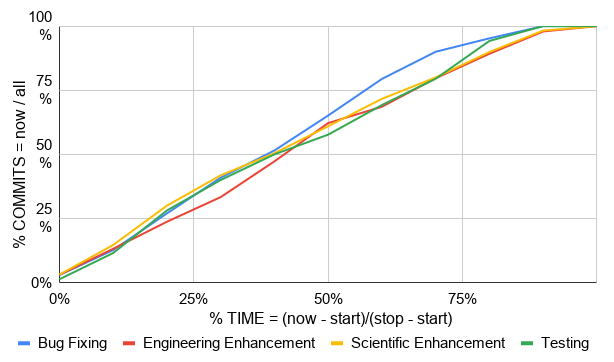
\includegraphics[width=\linewidth]{img/belief1_1.png}
\caption{{\bf BELIEF1 Result,} 
Median percent  of total commits seen
at 10,20,30,..100\% of 
the time these projects were
documented in Github. Data from the 59
projects of Table~\ref{tbl:all_projects}.
Note
that all commit types occur
at a similar, and near constant,
rate, across the lifetime of a project.}\label{fig:belief1}

\end{figure}



\subsection{Verification and validation}~\\
 \textit{\underline{Belief:}} 
Verification and validation in software development for CS is difficult and strictly scientific \cite{carver07_environment, kanewala13_testing, carver06_hpc, Prabhu11_cssurvey, basili08_hpc}.

\noindent \textit{\underline{Rationale:}} 
According to Carver et al.~\cite{carver07_environment},
CS validation means ensuring the mathematical model matches the real world; while CS verification means ensure the computational model matches the mathematical model. Past studies argued that verification and validation of scientific software should be  difficult for  several reasons:

\bi
    \item Lack of suitable test oracles \cite{kanewala13_testing},
    \item Complex distributed hardware environments with no comparable software \cite{basili08_hpc},
    \item Scientists often suspect that the problems of the software is the results of their scientific theory~\cite{faulk09_secs},
    \item Lack of physical experimentation and experimental validation is impractical \cite{carver07_environment}. 
\ei

% \begin{table}[!t]
% \caption{Labels of development types, generated via manual cross-inspection on 4000 random bug-fixing commits of 20 CS projects.
% }\label{tbl:everything}
% \vspace{3mm}

% \begin{center}
% %\begin{threeparttable}
% %\vspace{-10pt}
% %\resizebox{!}{0.2\linewidth}{
% %\setlength        abcolsep{10pt}
% \vspace{-10pt}\begin{tabular}{l|c|c}
%  \multicolumn{1}{c|}{} & \multicolumn{1}{c|}{Absolute} & \multicolumn{1}{c}{Percentage}\\
% \hline
% Bug Fixes & 764 & 19\% \\
% Scientific Enhancement & 1031 & 26\% \\
% Engineering Enhancement & 1134 & 29\% \\
% Testing & 608 & 15\% \\
% Other & 475 & 12\% 
% \end{tabular}
% %}
% %\end{threeparttable}
% \end{center}
% \vspace{3mm}
% \end{table}

\hspace{-10mm} \begin{figure}
     \centering
     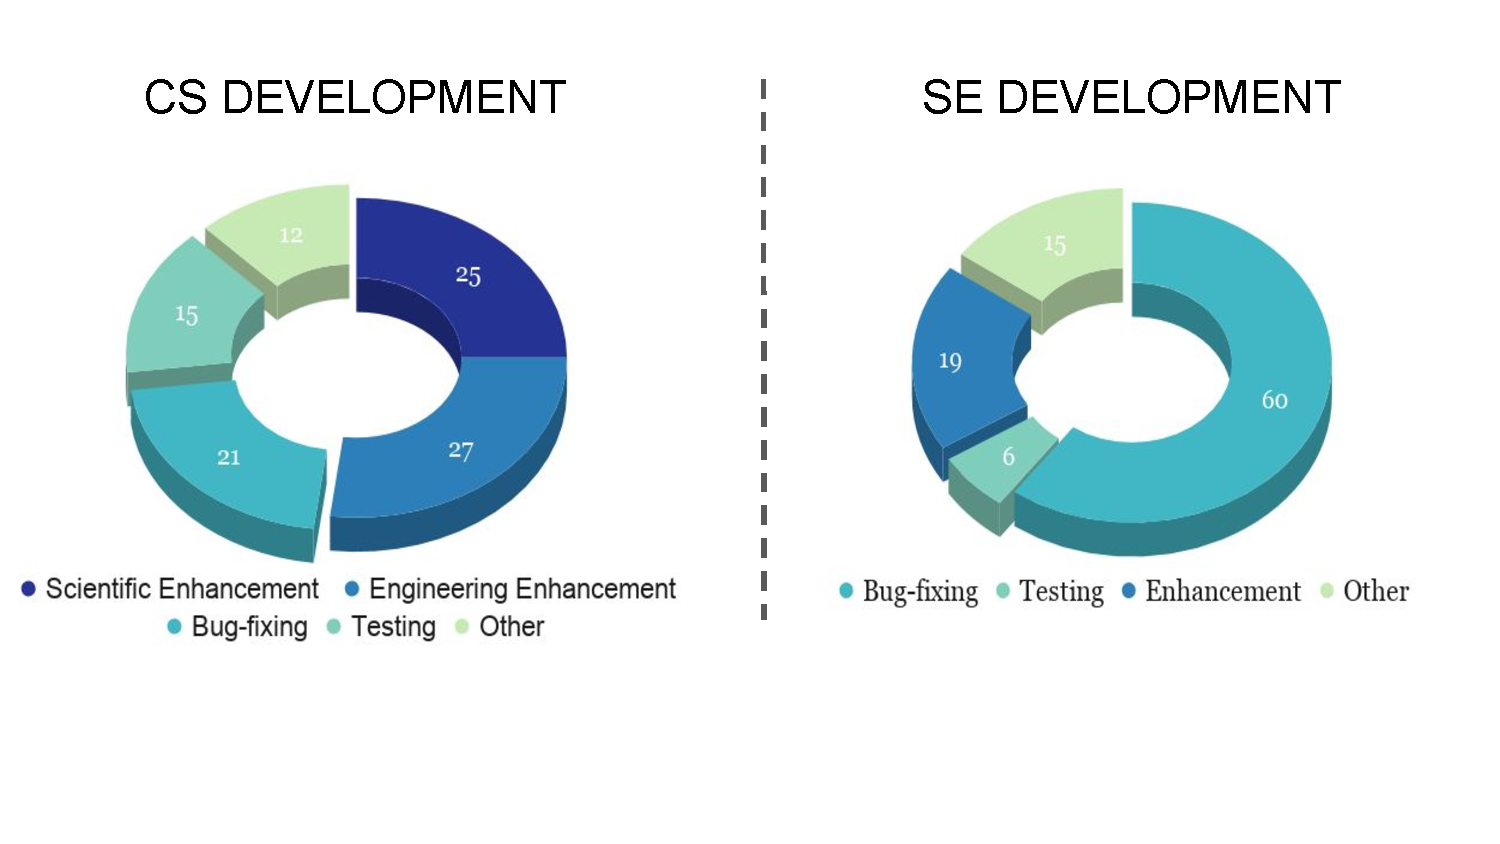
\includegraphics[width=1\linewidth, height=4.5cm]{img/activities.pdf} 


     \caption{Distribution of development activities within CS (left) and SE (right) projects within our sample.}
     \label{fig:SE_activities}
 \end{figure}


\begin{table}[!t]
\caption{Labels of testing type commits from the labeled Testing commits.}\label{tbl:testing}
\begin{center}
\vspace{-10pt}\begin{tabular}{l|c|c}
 \multicolumn{1}{c|}{} & \multicolumn{1}{c|}{Absolute} & \multicolumn{1}{c}{Percentage}\\
\hline
Science & 289 & 47\% \\
Engineering & 146 & 24\% \\
Other & 173 & 29\% 
\end{tabular}
%}
%\end{threeparttable}
\end{center}
\vspace{3mm}
\end{table}



\noindent \textit{\underline{Modeling Assumptions:}} See  above, in \S\ref{model}

\noindent \textit{\underline{Prediction:}}
Verification and validation in CS
``difficult'' if the observed CS effort in this area
is much larger than some known baseline.  As to ``strictly scientific'', we should see far more ``scientific
testing'' that otherwise (e.g. ``engineering testing''). 

\noindent \textit{\underline{Result:}}
It is easy to show that CS software verification and validation is heavily  focused on scientific issues.
Table \ref{tbl:testing} shows that ``scientific testing'' is the largest type of commit in our labeled Testing commits sample (at 45\%).  Far less effort is spent on ``engineering testing'' (only 17\%). 


As to showing the CS verification and validation is ``more difficult'',
the right chart in Figure \ref{fig:SE_activities} shows the 6\% percent  of commits in standard SE projects
 associated with testing.  This data comes from a recent study \cite{tu2019better} of the top-20 highly starred from Github that satisfy our sanity checks of Table~\ref{tbl:sanity}.
Since 15\% is 2.5 times larger than 6\%, for verification and validation, 
far more effort is being spent in CS projects than SE.





% Among all the defects fixing, the scientific and engineering defects are at the same rate. Yet, the testing focuses solely on scientific aspect, almost three times (45\%/17\%), more than engineering testing. In a sense, scientists solely believe that the software is defected due to their science understanding when transferring that to source code while overlooking the engineering aspect. Yet, it is understandable because scientists have a lot of responsibilities (read and write papers, grants, give presentations, develop scientific models, etc) so they can only focus on testing on what they good at, i.e. scientific models. It is possibly useful for the community to incorporate automated SE testing tools for CS projects. 

\begin{RQ}
\textit{\underline{Conclusion:}}
We \textbf{endorse} the belief that within CS, software development's verification and validation, are difficult and mostly concerned with scientific issues. At least in comparison with SE's V\&V, CS's V\&V are far more difficult.
\end{RQ}  

\noindent \textit{\underline{Discussion:}} This result is somewhat strange since it runs counter to standard beliefs in the SE literature (e.g. Brookes argues that unit tests and systems tests will consume half the time of any project~\cite{brooks1995mythical}). We conjecture that the larger V\&V effort in SE  is due to the nature of CS problems:
%CS software is more grounded in unchanging physical realities that standard SE software:

\bi
\item CS software is written to correspond to solve endless nature's problems (most are beyond human's understanding) with the requirements are not known up front and software's state are incrementally improved. 
\item SE software is written to handle more day to day operations with it's focus on production (shipping to the customer/business). 
\item CS V\&V have to cover both scientific and engineering concerns while SE V\&V at some points would mature to only focusing on verification. 
\ei 

Specifically, by looking at the \textit{Testing} and \textit{Bug-fixing} attributes from Figure \ref{fig:SE_activities}, the bug-fixing activities from SE software development are almost three times as in CS which is the direct result from testing 2.5 times less than CS. Essentially, the \textit{less} developers test, the \textit{more} bugs developers have to fix. After shipping the software, SE developers are more reluctant to test the software while for CS developers, scientific software research and development might be an endless journey.

Hence, it is not surprising CS software requires more verification and validation effort than SE software because of the research nature over production nature and the problem it addresses are more dynamic and  ``tests'' need to be a higher level and refer back to some core physical properties as defined
by scientific theory.  

%\item CS software is written to correspond to physical phenomena, the nature of which may never change (e.g. the atomic weight of iron).
%\item
%the highly starred projects in Github) is written to correspond to an ever-changing ecology of platforms, tools, user expectations, and newly-arrive AI algorithms, etc etc.   
%Hence, it is not surprising  SE software requires more verification and validation effort than CS software since the problem it addresses are more dynamic.
%\ei

%Whatever the reason, 
%note that this result calls for a different kind of testing device in CS.  In standard SE, a ``test'' can be something as simple as a unit test (checking if, for example, that subtrees remain in sorted order after insertion).
% But in CS, ``tests'' need to be a higher level and refer back to some core physical properties as defined
% by scientific theory.  


% \noindent \textit{\underline{Threats of Validity:}} CS developers are good at contributing relevant code to the system that less likely to introduce the bugs which make them more confident to spend less time on maintenance. 
 

 

%  \subsection{Formality}~\\
%  \noindent \textit{\underline{Claim:}} Overly Formal Software Processes Restrict Research \cite{easterbrook_cs, segal07_problem, carver07_environment, segal08_ss}.

%  \noindent \textit{\underline{Rationale:}} 
% Scientific software development is deeply embedded into the scientific methods and research fashion where developers will find traditional software development processes with big design upfront (e.g. waterfall approach) very challenging \cite{easterbrook_cs}. 
% As scientific software is evolving continuously no clear-cut requirements analysis, design, or maintenance phases can be discerned \cite{segal07_problem}. Therefore, instead of established SE processes, scientists apply an informal, nonstandard process. 

 
% The scientists regard their informal software process as necessarily following
% from applying the scientific method to scientific reasoning with the help of computing. The process itself has a lot of resemblances with the agile methodology. The process involved:
%  \begin{enumerate}
%      \item starts from a scientific problem and the necessary software or application could be required to solve
%      \item a prototype is developed and continuously improved, guided
% by the questions ``Does it do what I want?'' and ``Does it help solve the scientific problem at
% hand?''
%     \item cursory testing
%     \item modifications till plausible outputs are achieved.

%  \end{enumerate}

%  \noindent \textit{\underline{Result:}}

\begin{table}[!t]
\caption{Language Usage within sample of quality CS projects. 
}\label{tbl:language}
\vspace{3mm}
\begin{center}
%\begin{threeparttable}
%\vspace{-10pt}
%\resizebox{!}{0.2\linewidth}{
%\setlength        abcolsep{10pt}
\vspace{-10pt}\begin{tabular}{l|c|c}
 \multicolumn{1}{c|}{} & \multicolumn{1}{c|}{Absolute Count} & \multicolumn{1}{c}{Percentage}\\
\hline
Other & 3 &  5\%  \\ 
Javascript	& 2 & 3\% \\ 
C &	3 & 5\% \\ 
Java	& 5 & 9\% \\ 
Fortran	& 6 & 10\% \\
C++	& 17 & 29\% \\
Python & 23 & 39\% 
\end{tabular}
%}
%\end{threeparttable}
\end{center}
\vspace{3mm}
\end{table}



\section{Limitations of Computer Hardware}

% In this section, we discuss characteristics of software development in
% computational science that are due to limitations regarding available computing
% resources and their efficient programming. 

\subsection{Programming Languages, Technologies, and SE Methods }
In this subsection we explore a combination of beliefs 2b and 3f.

\noindent \textit{\underline{Belief:}} Computational scientists prefer
 ``older''-style programming languages and technologies while disregarding most of the newer SE methods~\cite{basili08_hpc, carver07_environment, Prabhu11_cssurvey, kendall05_C, ragan14_pythoncs}.   

\noindent \textit{\underline{Rationale:}} CS Scientists are skeptical of modern SE methods and new technologies/languages.
Given their success with   older-style languages
(Fortran and C).  This is based on several factors: 
\begin{itemize}
    \item A decades-long commitment with these older-style languages on high-performance computing platforms \cite{faulk09_secs}.
     \item A  belief that the extra features of the newer
     languages needlessly conflate functionality that can be
     more easily implemented in (e.g.) one line of ``C'' macros  \cite{sanders08_risk}. 
    \item A prejudice against the never languages or a perception that the scientists would not find then useful \cite{Prabhu11_cssurvey}.  
\end{itemize}

\noindent \textit{\underline{Modeling Assumptions:}} 
\bi
\item Old languages/technologies: based on the literature review of Johanson et al.~\cite{johan18_secs}, we say that ``C''
and ``Fortran'' are the older, most established languages in the CS community. 
Everything else, we will call ``newer languages''.
\item Modern SE practices are associated with automating tests and deployment continuously (e.g. Travis CI) 
\ei

In order to assess this combined belief (2b and 3f), the usage of language per project within the sample (Table \ref{tbl:language}) is recorded along with the usage of Travis CI.

\noindent \textit{\underline{Prediction:}} We would endorse this belief if (1) most the languages used by the CS projects are ``older'' style and (2) most CS projects do not adopt the usage of Travis CI. 


\noindent \textit{\underline{Result:}} 
``C'' and ``Fortran'' are just 15\% of our sample
while most of our projects use ``newer''
languages (where ``new'' is defined by Johanson et al.~\cite{johan18_secs}).

We have other evidence that CS developers might be more open to newer
technologies than suggested in the current literature. Through looking over
our 59 projects, we observe that 43 of them (73\%) have active
Travis CI connections. Travis CI is a standard tool within the continuous deployment community  that run tests as a side-effect
of any commit being written to Github. 

\begin{RQ} 
\textit{\underline{Conclusion:}} We \textbf{doubt} the belief that 
CS Scientists are skeptical of modern SE methods and new technologies/languages.
\end{RQ}
 
 \noindent \textit{\underline{Discussion:}} While this result is at odds
 with  numerous papers~\cite{basili08_hpc, carver07_environment, Prabhu11_cssurvey, kendall05_C, ragan14_pythoncs}. We explain our novel findings as follows. 
 Most of the papers that endorse this view come from before the recent Silicon Valley boom. In our discussions with postdocs and PhD students working on CS projects,
 we noted that they are very well aware the salaries they might earn if,
 they moved on to software companies later in life.
 They understand that the prerequisites for a career move would be a deep understanding of popular tools used by contemporary agile software companies. Hence, it is perhaps not so surprising that we report here a widespread use of modern software techniques in CS.
 
 
\subsection{Domain Logic and Implementation Details}~\\
\noindent \textit{\underline{Belief:}} Intermingling culture of domain logic and implementation details within scientific software development \cite{faulk09_secs}.


\noindent \textit{\underline{Rationale:}} Scientific software development is different from traditional software development due to the inseparable relationship of the usage of older programming languages and software with the focus of scientific models performance. The developers of such software should be, but difficult to be, proficient in both aspects. This leads to researchers having difficulty in evolve one aspect independently. 

\noindent \textit{\underline{Modeling Assumptions:}} During scientific software development,
\bi
\item domain logic addresses computational models, i.e. core science, understanding (referenced as scientific enhancement activities). 
\item implementation details address coding/building the tool up to solve scientific problem (referenced as engineering enhancement activities). 
\item the distribution and the rate across the project development of both types of enhancement activities serve as the indicator to characterize the nature of their development within the project. 
\ei

\noindent \textit{\underline{Prediction:}} If domain logic and implementation details are intermingled/inseparable during the development of scientific software, then (1) both scientific and engineering enhancement contribution distribution should be the same or have a very small difference from each other and (2) the scientific and engineering enhancement rate should be growing synchronously.  

 \noindent \textit{\underline{Result:}}  Across the enhancement type commits from the sample (from Figure \ref{fig:SE_activities}), 26\% enhancement commits focusing on the core science while the rest 29\% enhancement commits focusing on the quality of the code. The absolute difference between two type of enhancement activities is small (3\%). 
 
Moreover, from Figure \ref{fig:belief1}, the rate of commits of engineering and scientific enhancement activities are observed to grow synchronously across the project lifetime.   
 
\begin{RQ}
\textit{\underline{Conclusion:}} (1) the small difference of the two type of enhancement activities percentage and (2) the synchronous growing rate of both activities demonstrate our \textbf{endorsement} for this characteristic that developers of scientific software spent their time and efforts to enhance both the core science and the code evenly in parallel.
\end{RQ}

\begin{figure}
    \centering
    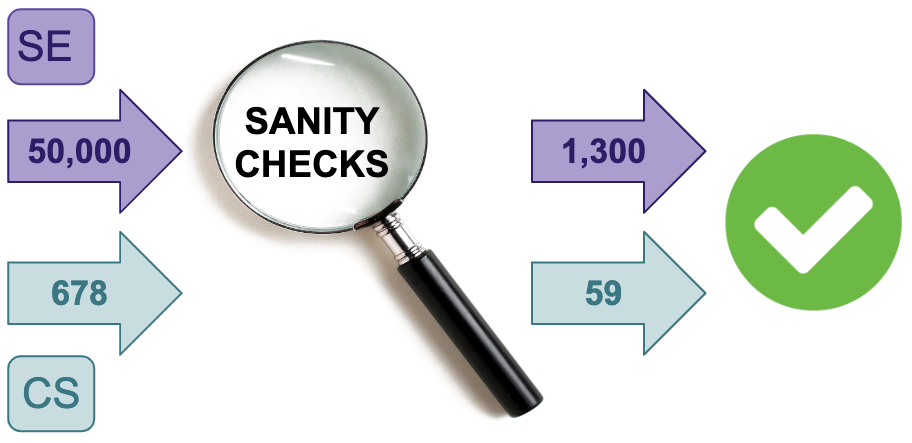
\includegraphics[width=\linewidth]{img/sanity.png} 
    \caption{The SE (cyan) and Computational Science (magenta) projects count number of before and after sanity checks.}
    \label{fig:sanity}
\end{figure}

\begin{figure*}[!t]
\vspace{5pt}
\centering 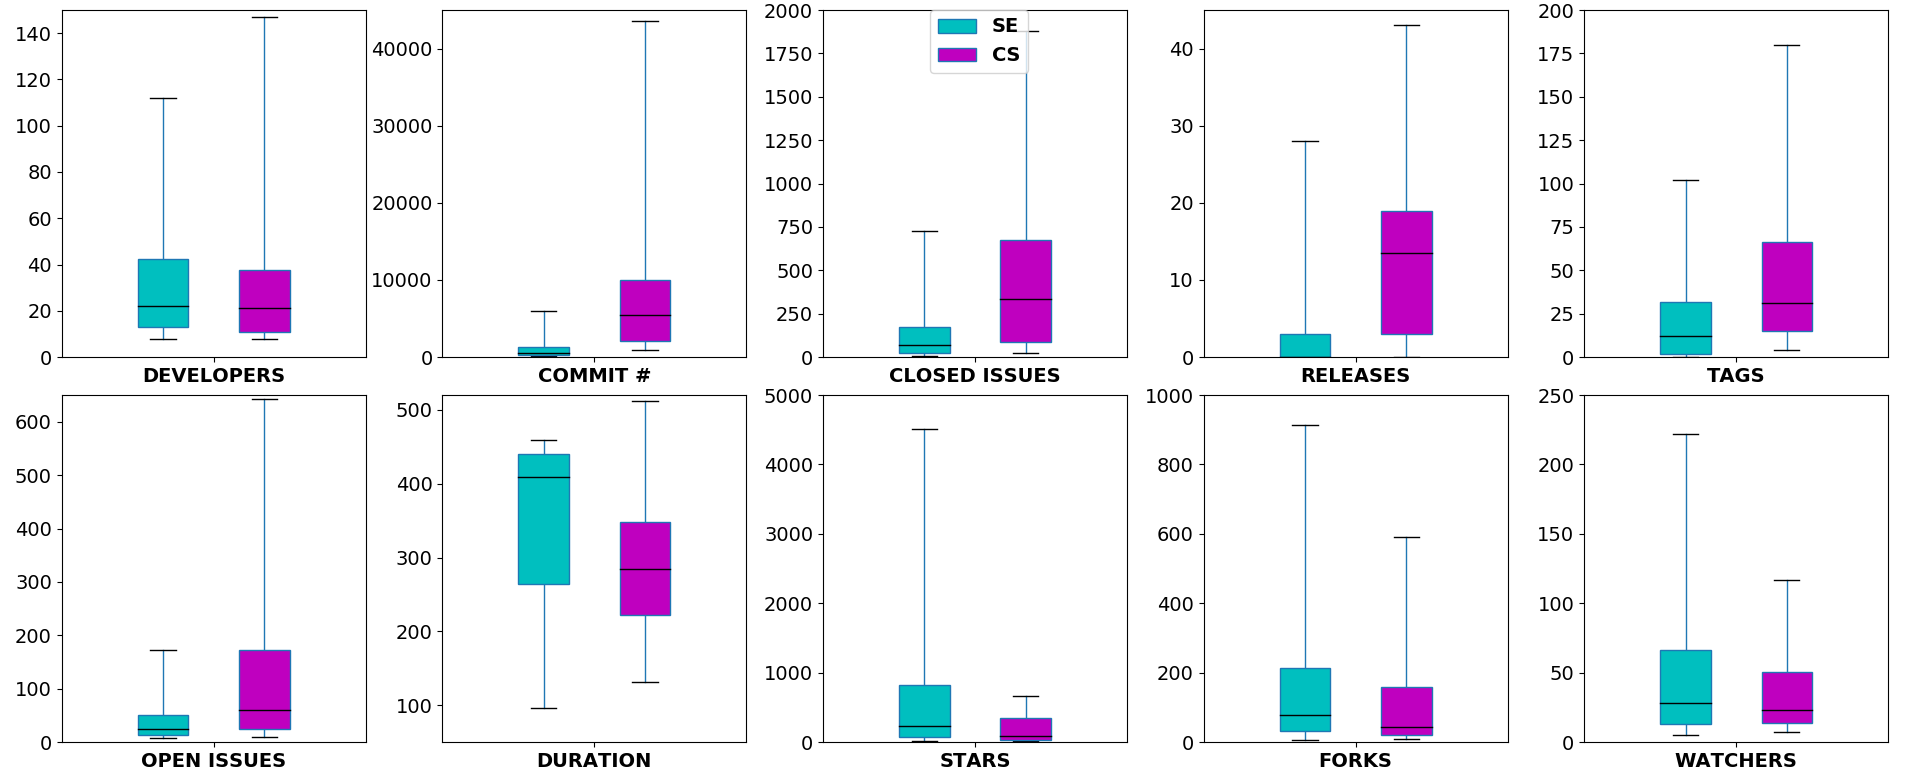
\includegraphics[width=\linewidth]{img/comparison.png}
\caption{Github statistics comparison of 1,000+ SE projects (Cyan) \& 59 CS projects (Magenta).}\label{fig:comparison}
\end{figure*}    


\section{Cultural Environment of Scientific Software Development}

% The characteristics that are listed in this section result from the cultural
% environment in which scientific software development takes place. This
% environment is shaped, for example, by the training of computational scientists
% and the funding schemes of scientific research projects. 

\subsection{SE Training} ~\\
\noindent \textit{\underline{Belief:}} Few CS scientists are trained in SE \cite{segal07_enduser, basili08_hpc, carver13_perception, easterbrook_cs, sanders08_risk}.

\noindent \textit{\underline{Rationale:}} Not many of scientists have SE knowledge or skill due to (1) SE are only considered as ``techniques'', a means to an end during the development of scientific software \cite{sanders08_risk} and (2) learning SE is perceived as an excessive demand \cite{boyle09_lessons}. 

\noindent \textit{\underline{Modeling Assumptions:}} training in SE is indicated by
\bi
\item the general quality of the software (e.g. the number of projects that pass the sanity checks)  
\item the adoption of SE practices (e.g. incremental development style) can be inferred by the distribution of different software development metrics in relation to each other.  
\ei

\noindent \textit{\underline{Prediction:}} If the belief is valid, then the proportion of the number of projects passed the sanity checked after over the number of all the projects of SE should be notably higher than the same proportion of CS. We also should not be able to derive any modern SE process practices from the software development metrics distribution of the CS projects development from Github. 

\noindent \textit{\underline{Result:}} In order to assess this belief, we first checked the number of projects between given CS ones and random 50,000 sampled SE ones after the sanity checks (from Table \ref{tbl:sanity} and mentioned in \S2.1) to make sure that they are more than just ``hobby'' projects as Figure \ref{fig:sanity} showed. We can see that after the sanity checks, the proportion of quality projects that are in CS community is 4  times higher than the quality projects that are in SE community (the calculation justification is offered right below). In another word, CS developers are more serious about their software development.  

\hspace{-10pt}\scalebox{1.1}{$\frac{CS\_post\_pre\_sanity\_rate}{SE\_post\_pre\_sanity\_rate} = \frac{\frac{CS\_post\_sanity}{CS\_pre\_sanity}}{\frac{SE\_post\_sanity}{SE\_post\_sanity}} = $} \scalebox{1.5}{$\frac{\frac{59}{678}}{\frac{1,300}{50,000}} = $} 4  

Furthermore, we summarized the the Github statistics of 1,000+ projects within the ``Github showcase project'' as SE projects and 59 quality CS projects in Figure \ref{fig:comparison}. Beside the \textit{Developer} statistics, it is observed that they committed, closed issues, deployed/released, and tagged more than standard software engineers significantly while the projects duration are notably shorter. Scientific developers are found to work with SE process philosophies in mind: build software faster and in a more granular fashion than SE projects. This is also observed by the Figure \ref{fig:belief1} that the growing rate of Enhancement activities and others are synchronous across the project lifetime which indicates a more incremental development style, essentially agile philosophy.  


\begin{RQ}
 \textit{\underline{Conclusion:}} With both of these evidences, we \textbf{doubt} this belief that few computational scientists are trained in SE as scientific developers (1) are more serious in developing their software and (2) built their software faster in a more granular fashion.
\end{RQ}

\noindent \textit{\underline{Discussion:}} The view of training in SE for us is not solely about data structures and algorithm understandings (i.e. may not be even applicable when entering SE career in Sillicon Valley). It is about the real-world experience and intuitions that scientists can also pick up from working with colleagues (e.g. 1.a belief: requirements are not known upfront, agile philosophy). Similar to \S4.1's \textit{Discussion}, CS developers are well aware that SE skills are appealing to high-profile companies in the industry.  Moreover, we also offer additional evidence to doubt this belief in \S6.4 that CS novices and outsiders understand the source code than SE ones to contribute significantly less defects.  

\noindent \textit{\underline{Threats of Validity:}} 

\subsection{Terminology}~\\
\noindent \textit{\underline{Belief:}} Both SE and CS fields used different terminologies (or even languages) to describe the the things they do, sometimes, the same activity \cite{faulk09_secs, easterbrook_cs, boyle09_lessons}.

\noindent \textit{\underline{Rationale:}} SE and CS fields have developed in isolation with established distinct languages. As a result, the scientific programmers might have not realized they have re-invented or used existing SE techniques.

\noindent \textit{\underline{Modeling Assumptions:}} 
\bi
\item Terminologies are regarded here as how scientists describe their work in the commits documentation. 
\item The difference between using off-the-shelf SE method versus tuned method that learn the CS language to label CS commits is the indicator.
\ei

\noindent \textit{\underline{Prediction:}} If the belief is hold, then the off-the-shelf SE method will perform badly when labeling scientific development commits in comparison with with tuned method that learn the CS language.  

\noindent \textit{\underline{Result:}} Tu et al. \cite{tu2019better} demonstrated that SE and CS used different languages in development documentation as different backgrounds come different terminologies and the language usage. They noted that the difference is so large that SE method for identifying bug-fixing commits cannot be adapted without prior modified to CS community. Comparing to human, after tuning the SE method to learn the CS language, they were able to reproduce better ground truths than SE method. That better ground truths generated more quality prediction for defect predictors. Specifically, Table \ref{tbl:rq2aaa} compares predictive performance using CS method (tuned SE method to learn the CS language) and standard SE method. The treatments with more superior performance are denoted by gray color. Note that,
in the majority case 7 out of 9 projects for both G-score and $P_{opt}$20. 


\begin{RQ}
\textit{\underline{Conclusion:}} With this empirical study's straightforward result, we confidently \textbf{endorse} that the CS community utilizes a different language when describing/documenting their work. 
\end{RQ} 

\noindent \textit{\underline{Discussion:}}  Tu et al. \cite{tu2019better} indicated a few reasons how their work demonstrates that a different model to learn the language of CS during software development is important. In the case of labeling defective commits, they observed that over half of the commits message were (a) very short (almost three times shorter than CS ones on median) and (b) took the form of
``\textit{Bug X: [type\_of\_bug] description\_of\_the\_bug-fixing\_commit}''. Moreover, bug-fixing commits from standard SE projects (79\% in median)
are three to four times more likely than the median values seen in the CS software (23\%). Both of these suggest that SE project are more standardized and mostly in maintenance mode. It is more convenient  and  possible  to  catch  bug-fixing activities through a few keywords (e.g. bug, fix, error, etc). Whereas, CS developed their software in a more dynamic style with a different way to describe and document their work across the development that requires adaptation of the language in order to understand scientific software development. 

\begin{table}[!t]
\caption{Win percentages of G-score (left) and $P_{opt}20$ (right) from \cite{tu2019better}. Gray cells highlight the labeling method that were top-ranked most in that project by the statistical tests (in $P (W/N)$ format). Treatments: SE method (SE) and tuned SE method for CS (CS)}
\label{tbl:rq2aaa}

\small 

\resizebox{\linewidth}{!}{
\hspace{-10pt}\begin{minipage}{0.54\linewidth}
\begin{tabular}{r@{~}|r@{~}|r@{~}}
\multicolumn{1}{c|}{} & \multicolumn{2}{c}{\textbf{\% G-score Wins}} \\
\cline{2-3}
\begin{tabular}[c]{@{}c@{}} \textbf{Dataset} \end{tabular} & 
\multicolumn{1}{c|}{\textbf{SE}} & \multicolumn{1}{c}{\textbf{CS}} \\ \hline
PCMSOLVER &  \cellcolor{gray!20} 100 (1/1) & 0 (0/1) \\ 
AMBER &  \cellcolor{gray!20} 67 (2/3) & 33 (1/3) \\ 
HOOMD & 40 (2/5) &  \cellcolor{gray!20} 60 (3/5)\\ 
RMG-PY  & 40 (2/5) &  \cellcolor{gray!20} 60 (3/5)\\ 
ABINIT & 25 (2/8) &  \cellcolor{gray!20} 63 (5/8) \\ 
LIBMESH & 28 (2/7) &  \cellcolor{gray!20} 72 (5/7)  \\  
MDANALYSIS & 28 (2/7) &  \cellcolor{gray!20} 72 (5/7) \\ 
LAMMPS & 25 (2/8) &  \cellcolor{gray!20} 75 (6/8)\\
XENON & 17 (1/6) &  \cellcolor{gray!20} 83 (5/6)  
\\  
\end{tabular}  %
\end{minipage} \
\begin{minipage}{0.60\linewidth}
%\centering

\begin{tabular}{r@{~}|r@{~}|r@{~}}
\multicolumn{1}{c|}{} & \multicolumn{2}{c}{\textbf{\% $P_{opt}20$ Wins}} \\
\cline{2-3}
\begin{tabular}[c]{@{}c@{}} 
\textbf{Dataset} \end{tabular} & \multicolumn{1}{c|}{\textbf{SE}} & \multicolumn{1}{c}{\textbf{CS}} \\ \hline
PCMSOLVER &  \cellcolor{gray!20} 100 (1/1) & 0 (0/1) \\ 
XENON &  \cellcolor{gray!20} 50 (3/6) &  \cellcolor{gray!20} 50 (3/6)\\
MDANALYSIS & 43 (3/7) &  \cellcolor{gray!20} 57 (4/7)\\ 
LIBMESH & 14 (1/7) &  \cellcolor{gray!20} 57 (4/7)\\  
HOOMD & 40 (2/5) &  \cellcolor{gray!20} 60 (3/5)\\ 
LAMMPS & 25 (2/8) &  \cellcolor{gray!20} 63 (5/8)\\
ABINIT & 25 (2/8) &   \cellcolor{gray!20} 63 (5/8)\\
AMBER & 33 (1/3) &  \cellcolor{gray!20}  67 (2/3)\\
RMG-PY & 0 (0/5) &  \cellcolor{gray!20}  80 (4/5)
\\
\end{tabular}
\end{minipage}}
%\end{center} 
\vspace{10pt}
\end{table}

Further, this result also raises attention for the current bad research fashion of reusing and applying established work without critiques. As seen, off-the-shell SE standard methods did not apply well for CS development data. The methods need to be tuned to specialize how scientific researchers develop their software. 

\subsection{Value} ~\\
\noindent \textit{\underline{Belief:}} Scientific software in itself has no value but still it is long-lived \cite{faulk09_secs, segal07_enduser, easterbrook_cs, boyle09_lessons}.

\noindent \textit{\underline{Rationale:}}  It is due to the belief that software is a representation of the underlying scientific theory with no novelty value of for new scientific discoveries \cite{sanders08_risk}. 

\noindent \textit{\underline{Modeling Assumptions:}} 
\bi
\item CS software's value is associated with the popularity of the project on Github (open and closed issues, stars, watchers, tags, and forks)
\item Live of scientific software is associated with the Duration of the software on Github. 
\item In both case, the difference of the metric for SE versus CS is the indicator. 
\ei


\noindent \textit{\underline{Result:}} According to the Figure \ref{fig:comparison}, the number of \textit{Open \& Closed Issues} are higher in Computational Science projects than in SE projects. The similar distributions of \textit{Stars}, \textit{Forks}, and \textit{Watchers} between CS and SE projects indicated similar values are placed by the audiences for both types of software. We took an additional step by using Scott-Knott testing (from \S2.5)  to rank the two CS and SE population for each of those three metrics if they are statistically different or not. As suspected, CS projects are ranked statistically similar to SE projects for those three metrics. 

Meanwhile, the distribution of \textit{Duration} demonstrated that even when the scientists believed their software is long-lived, the actual Duration of their software development is observed, on average, to be significantly shorter, almost 75\%, of the \textit{Duration} of the SE software. Similar to \textit{4.3.1}, from our sample, CS projects' lives are shorter with a greater commit density than SE projects. It indicates that CS software are important to the scientific developers that they spend more efforts to actually understand their code and offer more relevant contributions to xthe project's development.   


\begin{RQ}
\textit{\underline{Conclusion:}} These statistics are clear signals helping us to \textbf{doubt} that CS software have no value but long-lived.  
\end{RQ}

\noindent \textit{\underline{Discussion:}} Scientific software is developed by mostly Ph.D students and postdocs that have high personnel turnover rates \cite{johan18_secs}. Moreover, due to grant-based funding schemes and research natures, long-term vision is discouraged with ``quick and dirty'' solutions are more likely to be favored \cite{boyle09_lessons} which leads to short-lived software. 

The result for value aspect may surprise some folks. However, a trend in software-based research for both scientific developers or professional end user is following the development of the projects and ultimately use such project to curate necessary data, baseline results, and integrated framework that are relevant to their studies. Hence, the signal is clear by observing the similar distribution of \textit{Stars}, \textit{Forks}, and \textit{Watchers} (i.e. for following) and the greater distribution of \textit{Open \& Closed Issues} (i.e. for using) from CS's metrics to SE's metrics. 


\noindent \textit{\underline{Threats of Validity:}} Software live-span here is only applicable to Github as a warehouse that store these CS projects. Older existing systems and commercial projects that are not housed on Github may actually been around longer (e.g. Gitlab or/and local facilities). The value aspect here is only applying to Github popularity but not in term of how useful they are to people in real life. Essentially, scale versus impact debate that requires a more thorough and possibly longitudinal study to investigate the importance of one project to another, to the community, and to the civilization/world (e.g. combat global warming). 

\subsection{Code Understanding} ~\\
\noindent \textit{\underline{Belief:}} Creating a shared understanding of ``code'' is difficult \cite{segal07_problem, carver06_hpc, Shull05_parallel, sanders08_risk}. 

\noindent \textit{\underline{Rationale:}} All scientists typically (1) do not produce documentation for the software they implement \cite{segal07_enduser, sanders08_risk} and (2) high personnel turnover rates in scientific software development \cite{carver06_hpc, segal07_problem}. As a result, it renders such a knowledge and skill transfer problem. 

\noindent \textit{\underline{Modeling Assumptions:}} 

\bi
\item Code understanding here is associated with how experts (heroes) and novices/outsiders (non-heroes) interacting through the code and commits comments with issues. 
\item The defects introduction rate gap between two types of developers and the difference between the defects introduction rate gap in CS versus SE community are the indicator for code understanding.  
\ei

\noindent \textit{\underline{Prediction:}} If the belief is hold, the defects rate of hero developers would be a lot lower than the defect  rate of non-hero developers and the defects  rate gap of CS community would be the same or wider than the gap of SE community.  


\begin{figure}[!t]
\hspace{-0.5cm}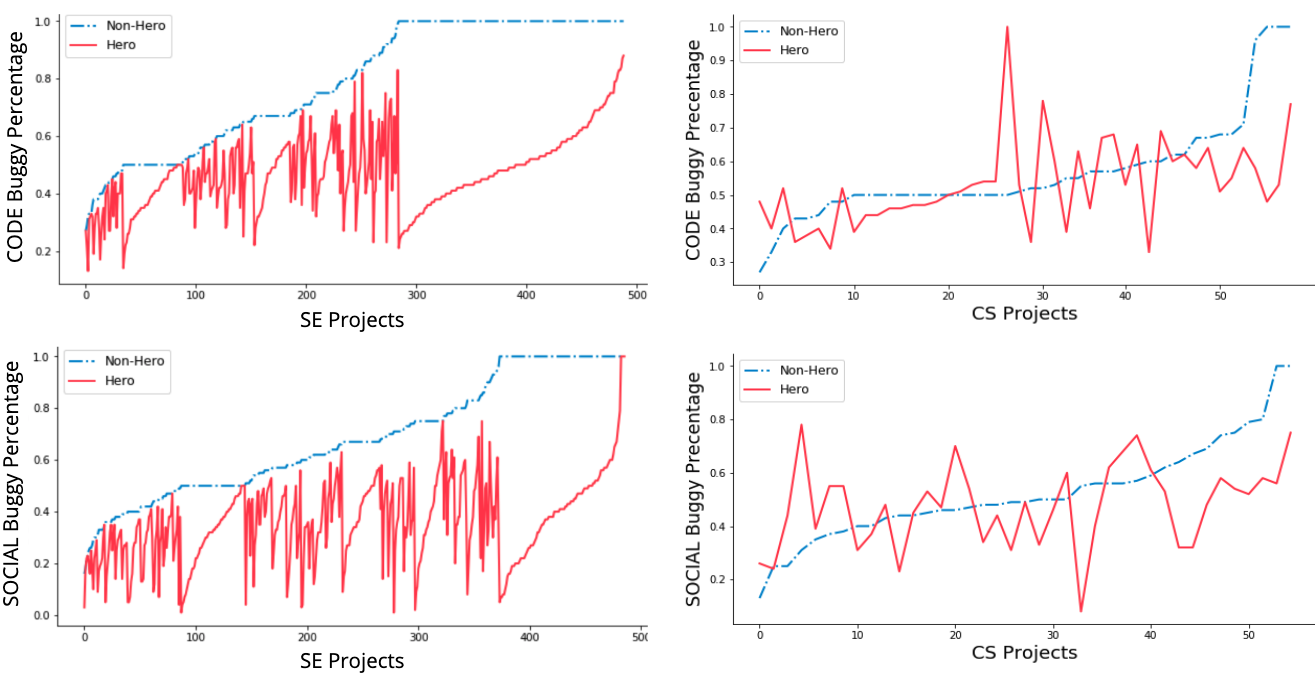
\includegraphics[width=1.05\linewidth, height=6cm]{img/heroes_1.png}
\caption{Defect rate introduced by hero and non-hero developers from developer code (top) and social (bottom) interaction perspective within SE projects (left) and CS projects (right). }\label{fig:heroes}
\end{figure}

\begin{table}[!t]
\begin{center}
\caption{The table summarizes of Figure \ref{fig:heroes} and stratifies the data according to 25th, 50th, and 75th percentiles of buggy percentages introduced through code and social interaction.}
\label{tbl:heroes}
\resizebox{1\linewidth}{!}{
\begin{tabular}{c|c|r@{~}|r@{~}|r@{~}|r@{~}|r@{~}|r@{~}}
& & \multicolumn{6}{c}{\textbf{Category}} \\
\cline{3-8}
&  & \multicolumn{3}{c|}{\textbf{SE Projects}} & \multicolumn{3}{c}{\textbf{CS Projects}}\\
\cline{3-8}
\textbf{Metric} & \begin{tabular}[c]{@{}c@{}} \textbf{Percentile} \end{tabular} & \begin{tabular}[c]{@{}c@{}} \textbf{Hero}\end{tabular} & \textbf{Non-Hero} & \begin{tabular}[c]{@{}c@{}} \textbf{Ratio}\end{tabular} & \textbf{Hero} & \textbf{Non-Hero} & \textbf{Ratio} \\ \hline

\multirow{3}{*}{\begin{tabular}[l]{c} \rotatebox[origin=c]{90}{\parbox[c]{1.5cm}{\centering code interaction}} \end{tabular}}  & 
25th & 52 & 67 & 1.3 & 46 & 50 & 1.09  \\ [3pt]
& 50th & 58 & 75 & 1.3 & 52 & 52 & 1 \\ [3pt]
& 75th & 53 & 100 & 1.9 & 60 & 60 & 1 \\ [4pt]
\hline
\multirow{3}{*}{\begin{tabular}[l]{c} \rotatebox[origin=c]{90}{\parbox[c]{1.5cm}{\centering social interaction}} \end{tabular}}  & 
25th & 52 & 67 & 1.3 & 39 & 36 & 0.92  \\[3pt] 
& 50th & 58 & 75 & 1.3 & 49 & 48 & 0.98 \\ [3pt]
& 75th & 53 & 100 & 1.9 & 61 & 57 & 0.93 \\ [3pt]
\end{tabular}}
\end{center}
\end{table}


\noindent \textit{\underline{Result:}} Menzies et al. \cite{majumder19_heroes} checked the heroes projects for both heroes and non-heroes contribution of defects within software development. They found that non-heroes introduced 1.3-1.9 times more bugs (25th-75th percentiles) in those projects. However, when the study is replicated for CS projects,  Figure \ref{fig:heroes} and Table \ref{tbl:heroes} indicated that 25th-75th percentile, non-hero developers introduced slightly higher than the amount of bugs introduced by hero developers (1-1.09 times). While fewer people (heroes) made most of the changes within the software development, non-experts and novices are able to contribute to the software development without causing a lot of bugs (in respect to developer dynamics in SE projects development).  

\begin{RQ}
\textit{\underline{Conclusion:}} At least, in the aspect of defect, we \textbf{doubt} that shared understanding of ``code'' is difficult within the CS community.
\end{RQ}

\noindent \textit{\underline{Discussion:}} Cai et al. \cite{cai19_debt} reported that after refactoring or adding a large amount of new functionality would cause a lot of defects to the software. Scientific software development is comprised of mostly features enhancement and new development (65\%) which makes the CS software even more likely to be defective in comparison to SE software (only 9\%). Even with CS projects are more prone to defects, CS non-hero developers are able to contribute relevant code that less likely to contribute bugs way less than SE non-hero developers.  

It is a call for action that the CS community should organize and encourage more novices and outsiders to contribute to the scientific software development. 

% \noindent \textit{\underline{Threats of Validity:}} 



\subsection{Code Reuse} ~\\
\noindent \textit{\underline{Belief:}} Little code being re-used \cite{segal07_problem, carver06_hpc, Shull05_parallel, sanders08_risk}. 

\noindent \textit{\underline{Rationale:}} 
Scientific developers have a history to not adopt or re-use the software developed by others or even their own. They fear that: 

\bi
\item the structural assumptions from the others would be too strict and narrow \cite{carver06_hpc, basili08_hpc}
\item most of the software is not built with comprehensibility requirement as the top priorities \cite{segal07_problem}
\ei

Therefore, scientists believe that their time and efforts can be more conserved by being spent on implementing the new libraries and framework instead of understanding the existing framework and code which might serve the same functions.  

\noindent \textit{\underline{Modeling Assumptions:}} Projects can reuse the code through calling the libraries/packages outside of it's own repository. The amount of external imports (EI) and files that have external imports (FEI) are indications to the reuse activities within the software. There are four attributes for this that we define: 

\bi
\item \textit{IF\_Ratio} = EI / Total\_\#\_of\_Files
\item \textit{ILOC\_Ratio} = EI / LOC (total number lines of code)
\item \textit{II\_Ratio} = EI / Total\_\#\_of\_Imports 
\item \textit{FF\_Ratio} = FEI / Total\_\#\_of\_Files
\ei

For all of them, the higher of the value the better reuse within their projects.  

\noindent \textit{\underline{Prediction:}} There are little code reuse within the CS community if for more than half of the attributes defined above, we should see SE projects perform statistically higher. 

\begin{table}[!t]
\begin{center}
\caption{Median and standard deviation (SD) summary for four attributes portraying the reuse state of CS and SE projects.}
\label{tbl:reuse}
\footnotesize
%\resizebox{1\linewidth}{!}{
\begin{tabular}{c|c|c|c}
\textbf{Metric} & \begin{tabular}[c]{@{}c@{}} \textbf{Project} \end{tabular} & \textbf{Median} & \textbf{SD} \\ \hline
\multirow{2}{*}{\begin{tabular}[l]{c} \rotatebox[origin=c]{90}{\parbox[c]{0.7cm}{\centering IF Ratio}} \end{tabular}}  & 
CS & 3.2 & 1.6  \\ [2pt]
& SE & 2.9 & 1.6 \\ [2pt]
\hline
\multirow{2}{*}{\begin{tabular}[l]{c} \rotatebox[origin=c]{90}{\parbox[c]{0.8cm}{\centering ILOC Ratio}} \end{tabular}}  & 
SE & 13\textperthousand & 9\textperthousand  \\ [2pt]
& CS & 10\textperthousand & 8\textperthousand \\ [3pt]
\hline
\multirow{2}{*}{\begin{tabular}[l]{c} \rotatebox[origin=c]{90}{\parbox[c]{0.8cm}{\centering FF Ratio}} \end{tabular}}  & 
CS & 86\% & 19\%  \\ [2pt]
& SE & 81\% & 19\% \\  [2pt]
\hline
\multirow{3}{*}{\begin{tabular}[l]{c} \rotatebox[origin=c]{90}{\parbox[c]{0.7cm}{\centering II Ratio}} \end{tabular}}  & 
SE & 70\% & 27\%   \rule{0pt}{2.5ex} \\  [1.5pt]
& CS & 55\% & 19\% \\  [1.5pt]
\end{tabular}%}
\end{center}
\end{table}

\noindent \textit{\underline{Result:}} Table \ref{tbl:reuse} summarizes the median and SD for both CS and SE projects. Notice that when SE or CS community have higher median value in the attribute, the SD is very high. Through Scott-Knott testing, SE projects rank statistically similar to CS projects for all of the reuse metrics. 

\begin{RQ} 
\textit{\underline{Conclusion:}} With the overwhelming result above, we \textbf{doubt} that there are little code reuse within CS software development, at least in comparison with the SE community. 
\end{RQ}

\noindent \textit{\underline{Discussion:}} This result is surprising with well-studied reasons priorly mentioned. Yet, CS software do share the common ground of utilizing numerical and computational techniques to solve the problems. It is more natural and convenient to adopt those open-source libraries for scientific calculation tasks such as linear algebra, differentiation, parallel computational framework, etc. 

Meanwhile, SE projects cover solutions for diverse range of fields instead of only science (e.g. finance, health, transportation, etc). This leads to coverage of many different frameworks and specialized software libraries with number of magnitudes higher than CS projects. It is less likely for SE to share any common interests or/and software to recycle. 

\noindent \textit{\underline{Threats of Validity:}} This analysis is limited to only the higher level of import activities and we did take a precaution step by making sure that the external libraries are being called later in the same file. However, we acknowledge that more in-depth analysis of the whole source code can be investigated with different types of clone (exact, renamed, near miss, and semantic) and different approaches (text-based, token-based, tree-based, metric-based, semantic and hybrid). The comparison of such approaches can lead to $O(n^{(m-1)})$ complexity with $n$ as the current section of codes within the project and $m$ is the number of the projects to compare to. This is an interesting and important direction for future work that is beyond the scope of this paper.  






%\subsection{External Validity}

%Methodology to understand the difference between software development domains in SE. Not our final conclusions or definitions, all are threatened by external validities but our conclusions are reproducible and our analysis can be repeated when new data arrives. 




\section{Conclusion}

The premise of the prior research \cite{johan18_secs} is underlying shortcomings of existing approaches for bridging the gap between SE and CS can be identified by the 13 recurring characteristics or beliefs. Through a quantitative investigation on 59 projects, we noticed the disconnection between the prior study's beliefs and the observed signals. Therefore, it is essential to update those deep-rooted beliefs accordingly.  Of those 13 beliefs,
we find that three cannot be assessed
with respect to the Github data.
Of the remaining,
we can only endorse for four of the ten beliefs.  


One of our findings include scientific developers might be more skilled and well capable of SE practices and knowledge than they believed. Because of the understanding/miscommunication gap, they have operated with SE philosophies unknowingly. Moreover, it is also a call for action that the CS community should organize for more space and encouragement to the novices and outsiders to contribute to software development. This work can serve as a proof of concept to challenge SE community (outside of Silicon Valley) to grow out of their comfort zone to also learn from CS community.  

As the nature of the CS software development is changing, instead of hastily applying off-the-self SE practices and knowledge, it is more useful to tailor SE methods for CS community. Software engineers can, therefore, help scientific software developers to tailor the existing SE practices and knowledge to better fit the needs of the scientific software developers.

Our study reiterates the important message that software development look different for CS. Even when testing and requirement are considered essential in SE community, they are not the center of attention within CS community due to their creation purposes. During scientific development, everything between from establishing project requirements and V\&V are important, i.e. new development and enhancement. 

The current work here lays out highlighted perspectives, quantitative evidences to clarify existing beliefs about scientific software development, and proposed partial solutions to the ``chasm'' between SE and CS communities as part of a path toward interdisciplinary of two fields. It leads to a new characterization of the nature of CS which, in turn, suggests prioritization for specialized supporting tools and updated debate in this active research area. 

% Therefore, more
% research on this topic is needed, especially to empirically evaluate the 
% gains in productivity and credibility achieved for scientific software by such
% SE approaches. 


\section{Acknowledgments}

This work was partially funded by an NSF CISE Grant \#1826574 and \#1931425.

\balance
\bibliographystyle{ACM-Reference-Format}
\bibliography{sample.bib}

\end{document}
